% !TeX spellcheck = pl_PL
\documentclass[a4paper,twoside]{article}
\usepackage{polski}
\usepackage[utf8]{inputenc}
\usepackage{graphicx}
\usepackage{amsmath}

\usepackage[unicode, bookmarks=true]{hyperref} %do zakładek
\usepackage{tabto} % do tabulacji
\NumTabs{6} % globalne ustawienie wielkosci tabulacji
\usepackage{array}
\usepackage{multirow}
\usepackage{array}
\usepackage{dcolumn}
\usepackage{bigstrut}
\usepackage{color}
\usepackage[usenames,dvipsnames]{xcolor}
\usepackage{pdfpages}


\setlength{\textheight}{24cm}
\setlength{\textwidth}{15.92cm}
\setlength{\footskip}{10mm}
\setlength{\oddsidemargin}{0mm}
\setlength{\evensidemargin}{0mm}
\setlength{\topmargin}{0mm}
\setlength{\headsep}{5mm}

\newcolumntype{M}[1]{>{\centering\arraybackslash}m{#1}}
\newcolumntype{N}{@{}m{0pt}@{}}

\graphicspath{ {./images/} }

\definecolor{nie}{RGB}{178,34,34}
\definecolor{tak}{RGB}{0,120,0}

% === Reset inkrementacji sekcji przy nowym parcie === %
\usepackage{titlesec}

\makeatletter
\@addtoreset{section}{part}
\makeatother
\titleformat{\part}[display]
{\normalfont\LARGE\bfseries\centering}{}{0pt}{}


\begin{document}
\bibliographystyle{plain}



\begin{titlepage}
\title{\huge Interfejsy w Systemach Komputerowych - ULTIMATE}
\author{\large SonMati \\ Ervelan \\ Doxus}
\maketitle
\end{titlepage}

%===============================================================================
%*** PYTANIA I ODPOWIEDZI ******************************************************
%===============================================================================
\part{Pytania i odpowiedzi}

\section{\textcolor{blue}{RS-232}}
\subsection*{Prawda/Fałsz}
\begin{itemize}
	\item \textcolor{nie}{RS-232 jest portem przeznaczonym do synchronicznej transmisji znakowej. Generator taktu odpowiedzialny za wyprowadzanie znaków typowo ustawiany jest na: 1200bd, 2400bd, 4800bd, 9600bd, 19200bd.} \\
	{\small \emph{RS-232 jest portem przeznaczonym do asynchronicznej transmisji znakowej. Da się sztucznie stworzyć synchroniczną transmisję.}}
	
	\item \textcolor{tak}{Linie kontrolne w interfejsie RS-232 to: DTR, DSR, RTS, CTS, RI, DCD. Pary DTR/DSR i RTS/CTS wykorzystywane są do realizacji handshake'u w połączeniach bezmodemowych.} \\ {\small \emph{Tak, te pary linii mogą być wykorzystywane do handshake podczas gdy RxD i TxD zajmują się przesyłem danych.}}
	
	\item \textcolor{nie}{Transakcja w systemie MODBUS składa się z zapytania (query) wysyłanego przez stację Slave i odpowiedzi odsyłanej przez stację Master.} \\
	{\small \emph {Jest odwrotnie - zapytanie wysyła Master, a odpowiedź odsyła Slave.}}
	
	\item \textcolor{nie}{W trybie transmisji ASCII znacznikiem początku ramki jest znak ':', a kooca ramki para znaków CR LF. W trybie transmisji RTU znacznikiem początku ramki jest znak 'Ctrl-A', a kooca para znaków CTRL-Y CTRL-Z.} \\
	{\small \emph{Zdanie jest poprawne dla ASCII. Dla RTU, znacznikiem początku i końca ramki jest przerwa o długości minimum 4T, gdzie T jest czasem trwania jednego znaku.}}
	
	\item \textcolor{nie}{Standard RS-232 transmituje znaki synchronicznie, bity w znakach [asynchronicznie]} \\
	{\small \emph{Ostatnie słowo ucięte, więc spekuluję że tak właśnie było napisane. To nieprawda, jest odwrotnie.}}
	
	\item \textcolor{tak}{Standard RS-422 pozwala na osiągnięcie szybkości 10MBodów na odległości 100m.} \\
	{\small \emph{IMO pozwala, na slajdzie 12 jest napisane że 10 Mbd przy zasięgu DO 100m - czyli 100m chyba też.}}
	
	\item \textcolor{tak}{Liniami kontrolnymi w RS-232 nie są linie TxD, RxD, SG.} \\
	{\small \emph{Owszem, TxD i RxD są liniami danych, a SG to po prostu masa.}}
	
	\item \textcolor{tak}{System MODBUS składa się z faz zapytania i odpowiedzi.} \\
	{\small \emph{Tak właśnie jest.}}
	
	\item {W systemie MODBUS}
	\begin{itemize}
		\item \textcolor{tak}{Obowiązuje master/slave.} \\
		{\small \emph{Pewnie, a w dodatku Slave'ów może być wielu.}}
		
		\item \textcolor{tak}{Prędkości transmisji wynoszą od 1200 do 19200bd.} \\
		{\small \emph{Jak najbardziej.}}
		
		\item \textcolor{tak}{Ramka w ASCII może mieć format 7N2 (lub np. 7E1, 7O1).} \\
		{\small \emph{Tak, patrz warstwa fizyczna MODBUS.}}
		
		\item \textcolor{tak}{Ramka w RTU może mieć format 8N2 *(lub np. 8E1, 8O1).} \\
		{\small \emph{Tak, patrz warstwa fizyczna MODBUS.}}
	\end{itemize} 
	
	
	\item \textcolor{tak}{W trybie transmisji RTU jest kontrola błędów CRC.} \\
	{\small \emph{Tak, jest elementem budowy ramki RTU.}}
	
	\item \textcolor{nie}{Bit kontrolny w RS-232 zależy od bitu danych i bitu stopu.} \\
	{\small \emph{Bit kontrolny słuzy do kontroli parzystości/nieparzystości, nie ma związku z bitem stopu.}}
	
	\item \textcolor{nie}{Za pomocą RS-232 możemy połączyć ze sobą 2 stacje DCE} \\
	{\small \emph{Połączyć możemy dwie stacje DTE, lub DTE z DCE. Dwie stacje DCE łączą się za pomocą łącza telefonicznego.}}
	
	\item \textcolor{tak}{W MODBUS kontrola błędów jest realizowana za pomocą LRC lub CRC.} \\
	{\small \emph{Tak, LRC wykorzystywane jest w trybie ASCII, CRC w trybie RTU.}}
	
	\item \textcolor{nie}{Do portu RS 485 można podłączyć tylko jedno urządzenie, ale za to obsługiwać go z dużo większą szybkością i na większą odległość niż jest to możliwe w przypadku interfejsu RS 232.} \\
	{\small \emph{Można podłączyć do 32 stacji.}}
	
	\item \textcolor{nie}{Format ramki w protokole Modbus jest następujący: znacznik początku ramki, adres urządzenia slave, adres mastera, pole danych, znacznik końca ramki.} \\
	{\small \emph{Opis nie pasuje ani do trybu ASCII, ani RTU}}
	
	\item \textcolor{nie}{RS 232 jest portem przeznaczonym dla asynchronicznej transmisji znakowej, realizowanej zazwyczaj w trybie dupleksowym, czyli dwukierunkowej transmisji niejednoczenej (naprzemiennej)} \\
	{\small \emph{Tryb dupleksowy jest równoczesny, to półdupleksowy jest niejednoczesny.}}
	
	\item \textcolor{tak}{W interfejsie RS 232 linie TxD i RxD służą do transmisji znaków, natomiast DTR, RTS to wyjścia kontrolne, a DSR, CTS, RI i DCD to wejścia kontrolne.} \\
	{\small \emph{Indeed}}
	
	\item \textcolor{tak}{Multipleksowanie urządzeń ze znakowym portem asynchronicznym pozwala na ich kontrolę poprzez jeden port RS-232.} \\
	{\small \emph{Żeby kontrolować kilka urządzeń z jednego portu potrzebny jest koncentrator. Jeśli "używanie koncentratora" równa się "multipleksowanie", to PRAWDA.}}
	
	\item \textcolor{tak}{Węzeł podrzędny w systemie MODBUS po wykryciu błędu w komunikacie wysyła potwierdzenie negatywne	do węzła nadrzędnego.} \\
	{\small \emph{W odpowiedzi pole to jest wykorzystywane do pozytywnego lub negatywnego potwierdzenia wykonania polecenia.}}
	
	\item \textcolor{tak}{Czy w trybie ASCII systemu MODBUS każdy bajt wysyłany jest jako znak z przedziału 0x00, 0xFF?} \\
	{\small \emph{Bajt dzielimy na 2 części i wysyłamy jako 2 znaki z przedziału 0-9 i Ah-Fh}}
		
	
\end{itemize}


\section{\textcolor{blue}{USB}}
\subsection*{Prawda/Fałsz}
\begin{itemize}
	
	\item \textcolor{tak}{Kontrola urządzenia USB odbywa się poprzez zapisy komunikatów do bufora o numerze 0 i odczycie informacji statusowych z bufora o numerze 0.} \\
	{\small \emph{Zgadza się.}}
	
	\item \textcolor{nie}{W przypadku błędu transmisji każda transakcja USB jest powtarzana, ponieważ niedopuszczalne jest przekazywanie danych przekłamanych.} \\
	{\small \emph{Transakcje izochroniczne nie są powtarzane w przypadku błędu transmisji.}}
	
	\item \textcolor{tak}{Hub nie dopuszcza ruchu full speed do portów, do których są podłączone urządzenia low speed.} \\
	{\small \emph{Tak, urządzenie lowspeed blokuje możliwość włączenia fullspeed na całym porcie.}}
	
	\item \textcolor{nie}{Reset portu USB polega na rekonfiguracji hosta, po której host zapisuje tablicę deskryptorów do urządzenia podłączonego do tego portu.} \\
	{\small \emph{Reset portu USB polega na rekonfiguracji urządzenia. W następującej procedurze enumeracji między innymi dochodzi do odczytu tablicy deskryptorów z urządzenia przez host.}}
	
	\item \textcolor{nie}{Typowa transakcja USB składa się z pakietów żądania i odpowiedzi, z których każdy potwierdzany jest osobnym potwierdzeniem.} \\
	{\small \emph{Typowa transakcja USB składa sie z pakietów token, data i handshake. Transakcje izochroniczne nie są potwierdzane.}}
	
	\item \textcolor{nie}{W systemie USB urządzenia zgłaszają żądania do hosta, który je kolejkuje i następnie obsługuje w kolejności pojawiania się zgłoszenia.} \\
	{\small \emph{Urządzenia nie zgłaszają żądania, tylko są odpytywane przez hosta. Host nie tworzy jednej kolejki, tylko w miarę możliwości stara się obsługiwać wszystkie urządzenia jednocześnie, równomiernie, zapobiegając zawłaszczeniu.}}
	
	\item \textcolor{nie}{W USB można połączyd kaskadowo do 5 hubów, korzystających z zasilania magistralowego} \\
	{\small \emph{Podłączyć je można tylko korzystając z zasilania zewnętrznego lub hybrydowego. Przy zasilaniu magistralowym zabraknie zasilania już na drugim hubie. Co więcej, należy mieć na uwadze maksymalne dopuszczalne opóźnienie sygnału, które przy przejściu przez 5 hubów jest osiągane - 350ns. Urządzenia podpięte do 5'tego huba mogą nie działać poprawnie.}}
	
	\item \textcolor{nie}{Mechanizm data toggle w USB służy do przywracania synchronizacji pomiędzy hostem i urządzeniem, utraconej na skutek wystąpienia błędów w pakietach danych.} \\
	{\small \emph{Mechanizm data toggle zabezpiecza przed utratą synchronizacji pomiędzy hostem i urządzeniem na skutek błędu w potwierdzeniu odsyłanym przez odbiorcę.}}
	
	\item \textcolor{tak}{Host kontroler USB komunikuje się z interfejsem magistrali USB urządzenia peryferyjnego za pomocą fizycznego kanału komunikacyjnego.} \\
	{\small \emph{Tak, używamy kabelka.}}
	
	\item \textcolor{nie}{Kamera internetowa może przesyłać obraz do komputera za pomocą transferu izochronicznego z szybkością LowSpeed w interfejsie USB.} \\
	{\small \emph{Z tabelk można wyczytać, że dla transferu izochronicznego nie można wykorzystać szybkości LowSpeed.}}
	
	\item \textcolor{tak}{Pakiety USB przesyłane z szybkością LowSpeed muszą byd poprzedzone pakietem preambuły} \\
	{\small \emph{Tak, jest on charakterystyczny dla pakietów przesyłanych z szybkością LowSpeed}}
	
	\item \textcolor{nie}{Urządzenie peryferyjne USB 2.0 może być podłączone do host kontrolera za pośrednictwem maksymalnie sześciu hubów.} \\
	{\small \emph{Aby spełnid normę (ograniczenie czasowe oczekiwania na odpowiedź), można podłączyd za pośrednictwem maksymalnie 5 hubów.}}
	
	\item \textcolor{nie}{Pole PID w pakiecie USB zabezpieczone jest 16-bitową sumą kontrolną CRC.} \\
	{\small \emph{Pole PID zabezpieczone jest 4-bitowym polem kontroli, będącym prostą negacją bitów pola PID.}}
	
	\item \textcolor{nie}{Do portu dolnego huba podłączane mogą byd tylko wtyki USB typu B.} \\
	{\small \emph{Tylko wtyki typu A.}}
	
	\item \textcolor{nie}{Transakcja dzielona w USB 1.1 składa sie z dwóch części: SSPLIT i CSPLIT.} \\
	{\small \emph{Takie czary dopiero w USB 2.0}}
	
	\item \textcolor{nie}{W przypadku połączenia USB HighSpeed wykonywane jest podparcie linii D- do Vcc za pośrednictwem rezystora 1,5k.} \\
	{\small \emph{Po podłączeniu urządzenia High Speed wpierw jest ono identyfikowane jako Full Speed, więc wykonywane jest podparcie linii D+ do Vcc za pośrednictwem rezystora 1,5k. Następnie, poprzez chirp ("dwierkanie") host i urządzenie ustalają, czy możliwa jest komunikacja w trybie High Speed. Jeśli tak, usuwane jest podparcie przez rezystor, a obwód zamykany jest terminatorami.}}
	
	\item \textcolor{nie}{W kodowaniu NRZI co sześć jedynek jest wstawiany bit synchronizacji "0".} \\
	{\small \emph{Pomieszane pojęcia. W kodowaniu NRZI nie występuje dodawanie bitu synchronizacji. Proces ten nazywa się bit stuffing. Zdanie było by poprawne, gdyby brzmiało np. W kodowaniu NRZI z bit stuffingiem co sześć.}}
	
	\item \textcolor{nie}{Transakcje kontrolna i przerwaniowa w USB 1.1 są transakcjami aperiodycznymi z gwarantowanym pasmem w ramach jednej mikroramki.} \\
	{\small \emph{Transakcja kontrola jest transakcją aperiodyczną. Transakcja przerwaniowa jest transakcją periodyczną.}}
	
	\item \textcolor{tak}{W kontrolerze OHC transakcje izochroniczne są porządkowane/kolejkowane w drzewo/strukturę drzewiastą.} \\
	{\small \emph{Tak, OHC wykorzystuje strukturę drzewa, a UHC tablicę wskaźników (listę podwieszaną).}}
	
	\item \textcolor{tak}{Standard USB 2.0 wymaga skręconych, ekranowanych kabli.} \\
	{\small \emph{Well, High speed all the way, więc wymaga}}
	
	\item \textcolor{nie}{Transfer kontrolny i przerwaniowy są transferami aperiodycznymi.} \\
	{\small \emph{Było podobne pytanie. Transfer kontrolny jest aperiodyczny, transfer przerwaniowy jest periodyczny.}}
	
	\item \textcolor{tak}{Wielowarstwowa architektura USB 2.0 składa się z 3 warstw.} \\
	{\small \emph{Tak - warstwa interfejsu magistrali USB, warstwa urządzenia USB, warstwa funkcji urządzenia}}
	
	\item \textcolor{tak}{W porcie USB dane są dzielone na transakcje.} \\
	{\small \emph{Dane w ramce są dzielone na transakcje, więc tak}}
	
	\item \textcolor{nie}{Hub podłączony do portu USB ma obciążalność 100uA.} \\
	{\small \emph{Hub podłączony do portu USB bez własnego zasilania (zasilanie magistralowe) ma obciążalnośd dla portów dolnych do 100mA na port (maksymalną 400mA na cały hub). Hub z zasilaniem zewnętrznym lub hybrydowym ma obciążalnośd do 500mA na port.}}
	
	\item {W systemie USB do mechanizmów kontroli danych należą:}
	\begin{itemize}
		\item \textcolor{tak}{Przełączanie pakietów danych} \\
		{\small \emph{Tzw. Data Toggle}}
		
		\item \textcolor{tak}{Wykrywanie braku aktywności na linii danych;}
		
		\item \textcolor{nie}{Zabezpieczenie znacznika SOF lub EOF} \\
		{\small \emph{Reakcją jest natomiast objęte wystąpienie fałszywego znacznika kooca pakietu (false EOP)}}
		
		\item \textcolor{nie}{kodowanie LRC} \\
		{\small \emph{Pakiety zabezpieczone są kodowaniem CRC.}}
	\end{itemize}
	
	\item \textcolor{nie}{Wydajnośd dolnego portu (USB 2.0) wynosi 500mA.} \\
	{\small \emph{Nie wiadomo. Zasilany Hub może wystawić te 500mA, ale niezasilany już tylko 100mA}}
	
	\item \textcolor{tak}{USB 2.0 ma parę przewodów ekranowanych.} \\
	{\small \emph{Taki upgrade.}}
	
	\item \textcolor{nie}{W kodowaniu NZR wstawia się dodatkowe bity synchroniczne.} \\
	{\small \emph{Dodatkowe bity synchroniczne wstawia się w kodowaniu NRZI}}
		
	\item \textcolor{nie}{Urządzenie USB 2.0 może zasygnalizować swoją niegotowość do zapisu danych z szybkością High-Speed wysyłając pakiet PING-NYET.} \\
	{\small \emph{Wychodzi na to, że niegotowość zgłasza samym NYET? Pyta – PING, odpowiada (niegotowość) NYET. I Tak cały czas, chyba że dostanie ACK. ACK – wykonanie transakcji OUT. NYRT – host kontynuuje wysyłanie zapytań PING}}
	
	\item \textcolor{nie}{W systemie deskryptorów urządzenia USB może wystąpić kilka deskryptorów urządzenia, konfiguracji, interfejsów I punktów końcowych.} \\
	{\small \emph{Deskryptor urządzenia może być jeden. Innych – konfiguracji, interfejsu, końcowych może być więcej.}}
	
	\item \textcolor{tak}{Hub USB ma przerwaniowy punkt końcowy, który wykorzystuje do powiadamiania hosta o podłączeniu	urządzenia USB do któregoś z jego portów dolnych.} \\
	{\small \emph{Chyba.}}
	
	\item \textcolor{nie}{Na wierzchołku wielopoziomowego, hierarchicznego układu deskryptorów USB znajduje się deskryptor konfiguracji.}
	{\small \emph{Na szczycie znajduje się pojedynczy deskryptor urządzenia.}}
	
	\item \textcolor{nie}{Transfer masowy I izochroniczny USB 1.1 są przykładami transferów aperiodycznych z zagwarantowanym pasmem w ramach jednej mikroramki.} \\
	{\small \emph{Izochroniczny jest periodyczny, masowy nie ma zagwarantowanego pasma (wg tabelki z	prędkościami)}}
	
	\item \textcolor{nie}{W deskryptorze konfiguracji USB jest jakiś pole statusowe, które mówi o maksymalnym poborze prądu. Dla wartości 50 urządzenie pobiera 50mA.} \\
	{\small \emph{Pole to jest tak skonstruowane, żeby wartość zmieściła się w jednym bajcie, ze skokiem co 2mA. Dlatego urządzenie, które zgłasza, że 50 może zasysać maksymalnie 100mA.}}
	
	\item \textcolor{nie}{Uszeregowanie transakcji w USB. Nie zależy od implementacji kontrolera.}
	{\small \emph{w OHC przerwaniowe są w strukturze drzewa, a w UCH listy podwieszanej, co ma wpływ na uszeregowanie (do sprawdzenia).}}
	
	
\end{itemize}

\section{\textcolor{blue}{IEEE 1394 Firewire}}

\section{\textcolor{blue}{IEEE-488 i SCPI}}


\pagebreak
\part{Opracowanie materiałów}

\section{RS-232 – szeregowy port znakowy}
	\subsection{Charakterystyka interfejsu RS-232}
		\subsubsection{Transmisja danych}
		Szeregowa, asynchroniczna transmisja znakowa w trybie półdupleksowym.\\Rodzaje transmisji:
		\begin{itemize}
			\item Szeregowa - sekwencyjne przesyłanie bitów w ustalonej kolejności (od LSD lub MSB) po jednej linii transmisyjnej.\\
			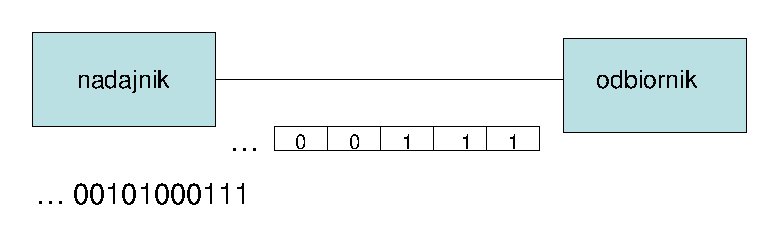
\includegraphics[width=9cm]{./wyklady/RS232_2_1.pdf}
			\item Równoległa - przesyłanie bitów słowa po przyporządkowanej każdemu bitowi linii transmisyjnej (bity przesyłane równolegle, słowa przesyłane szeregowo).\\
			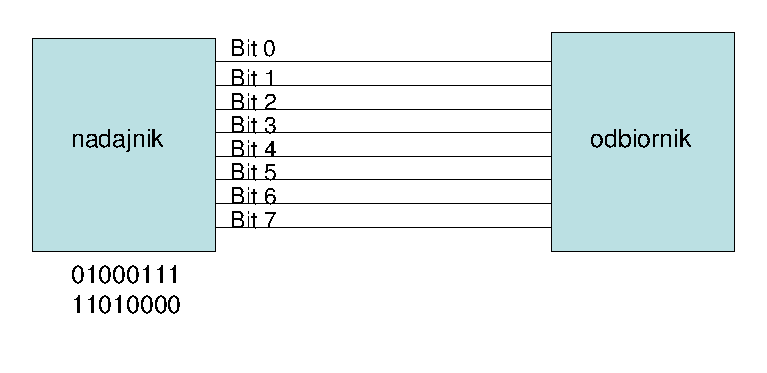
\includegraphics[width=9cm]{./wyklady/RS232_2_2.pdf}
		\end{itemize}
		\subsubsection{Jednostka informacyjna - znak}
		Format znaku\\
		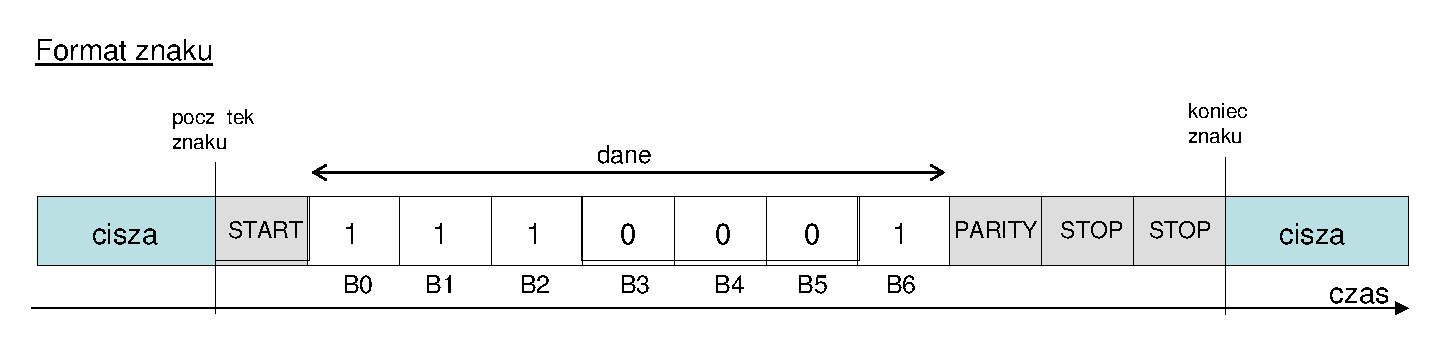
\includegraphics[width=10cm]{./wyklady/RS232_3_2.pdf}\\
		Bity kontrolne:
		\begin{itemize}
			\item \textbf{START} - znacznik początku (SOF)
			\item \textbf{PARITY} – bit kontroli poprawnosci znaku
			\item \textbf{STOP} – znacznik ko ca (1 lub 2 bity)
		\end{itemize}
		Bity danych:
		\begin{itemize}
			\item rozmiar pola 5, 6, 7 lub 8
			\item jako pierwszy przesyłany najmniej znaczący bit (B0)
		\end{itemize}
		\subsubsection{Rodzaje transmisji}
		\begin{itemize}
			\item \textbf{Synchroniczna} - elementy informacji wysyłane w takt zegara nadajnika.
			\item \textbf{Asynchroniczna} - wysyłanie elementów informacji niesynchronizowane zegarem nadajnika.
		\end{itemize}
		\subsubsection{Transmisja w RS-232}
		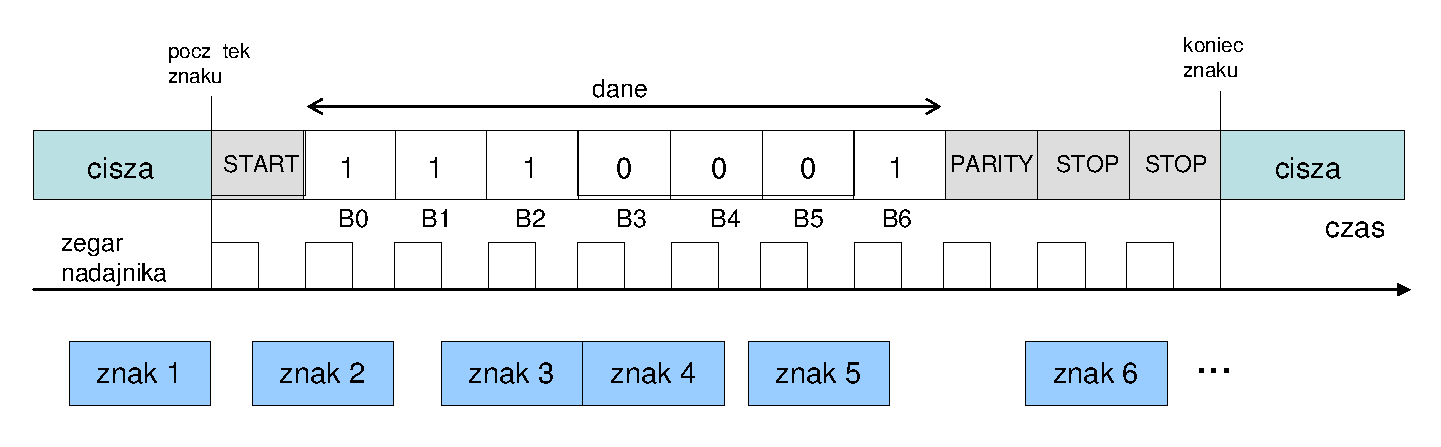
\includegraphics[width=9cm]{./wyklady/RS232_4_1.pdf}
		\begin{itemize}
			\item Synchroniczne wysyłanie bitów
			\item Asynchroniczne wysyłanie znaków
			\begin{itemize}
				\item Brak sygnału zegarowego określającego momenty wysyłania znaków
				\item Odstępy między znakami nieokreślone
			\end{itemize}
		\end{itemize}
		\subsubsection{Tryby transmisji}
		\begin{itemize}
			\item \textbf{Simpleksowa} - jednokierunkowa, z nadajnika do odbiornika
			\item \textbf{Półdupleksowa} - dwukierunkowa, niejednoczesna (w danej chwili czasu jedno urządzenia jest nadajnikiem, a drugie odbiornikiem)
			\item \textbf{Dupleksowa} - dwukierunkowa, jednoczesna (w danej chwili czasu oba urządzenia mogą spełniać rolę nadajnika lub odbiornika)
		\end{itemize}
	\subsection{Komunikacja DTE-DCE - sygnały w porcie RS-232}
	Komunikacja dwóch stacji DTE przez komutowane łącze telefoniczne.\\
	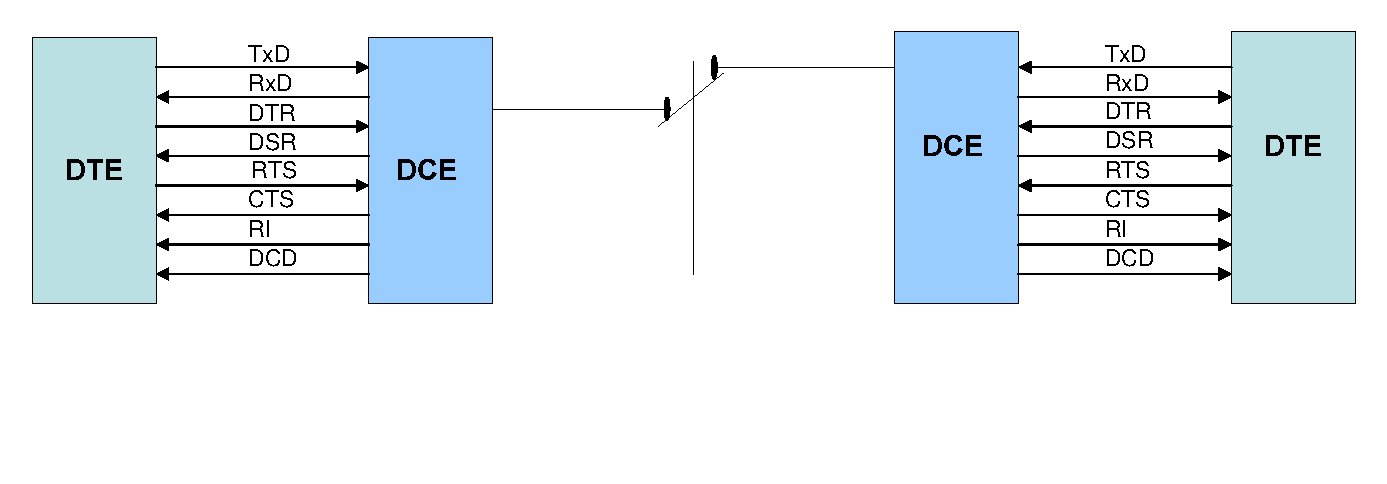
\includegraphics[width=12cm]{./wyklady/RS232_6_1.pdf}\\
	\begin{table}[h]
		\begin{tabular}{|c|c|c|}
			\hline
			\multicolumn{3}{|c|}{\textbf{Urządzenia}}                        \\ \hline
			\multicolumn{1}{|c|}{DTE} & Data Terminal Equipment      & Komputer           \\ \hline
			\multicolumn{1}{|c|}{DCE} & Data Communication Equipment & Modem              \\ \hline
			\multicolumn{3}{|c|}{\textbf{Linie} (sygnały)}                   \\ \hline
			TxD & Transmitted Data             & Dane nadawane      \\ \hline
			RxD & Received Data                & Dane odbierane     \\ \hline
			DTR & Data Terminal Ready          & Gotowość DTE       \\ \hline
			DSR & Data Set Ready               & Gotowość DCE       \\ \hline
			RTS & Request to Send              & Danie nadawania    \\ \hline
			CTS & Clear To Send                & Zgoda na nadawanie \\ \hline
			RI  & Ring Indicator               & Wskaźnik wywołania \\ \hline
			DCD & Data Carrier Detected        & Wykrycie nośnej    \\ \hline
			SG  & Signal Ground                & Masa sygnałowa     \\ \hline
		\end{tabular}
	\end{table}
		\subsubsection{Fazy pracy układu}
		\begin{itemize}
			\item Nawiązanie połączenia
			\item Transmisja danych
		\end{itemize}
		\subsubsection{Linie w złączu RS-232}
		\begin{itemize}
			\item Linie danych: TxD, RxD
			\item Linie kontrolne: DTR, DSR, RTS, CTS, RI, DCD
		\end{itemize}
	\subsection{Połączenie bezmodemowe DTE-DTE}
	Przykład połączenia dla transmisji dupleksowej.\\
	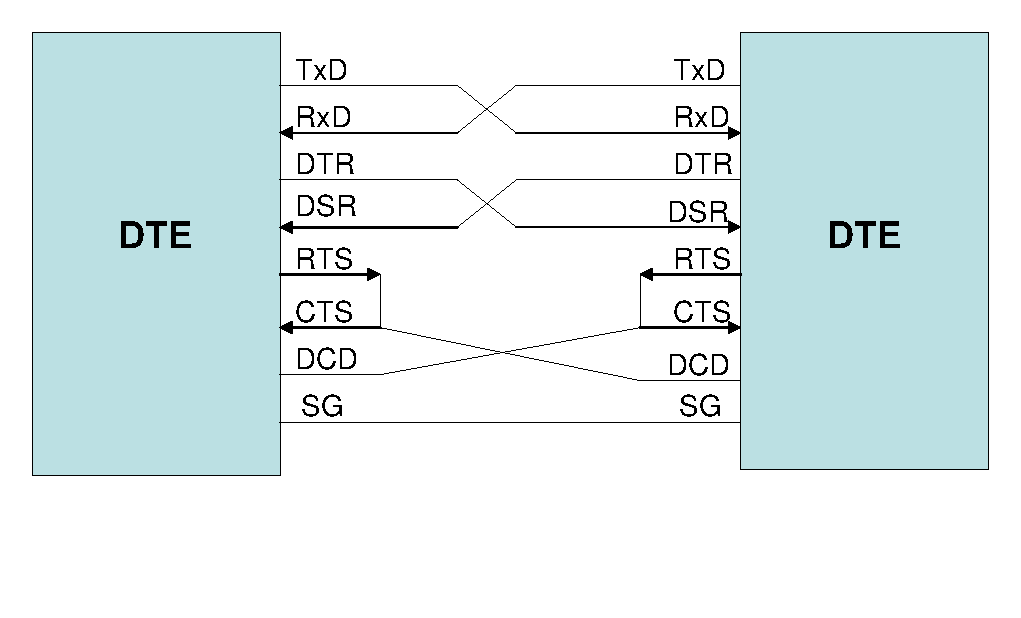
\includegraphics[width=9cm]{./wyklady/RS232_7_1.pdf}
	\subsection{Kontrola transmisji: handshake i protokół XON/XOFF}
		\subsubsection{Handshake}
		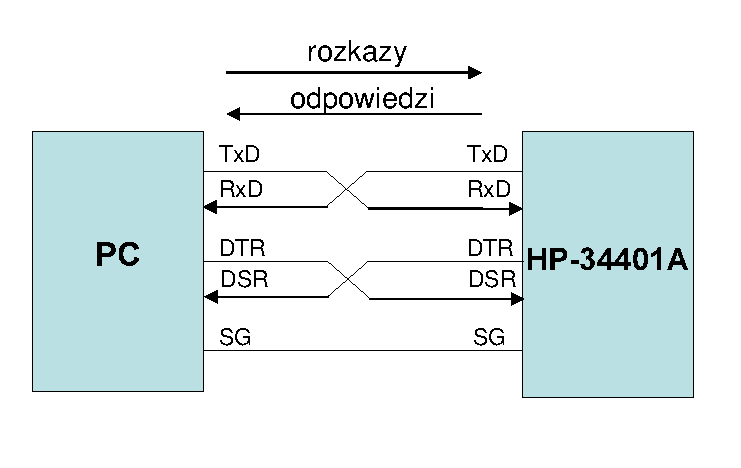
\includegraphics[width=9cm]{./wyklady/RS232_9_1.pdf}\\
		\begin{itemize}
			\item DTR = 1 - zgoda na nadawanie
			\item DTR = 0 - brak zgody na nadawanie
		\end{itemize}
		\subsubsection{Protokół XON/XOFF}
		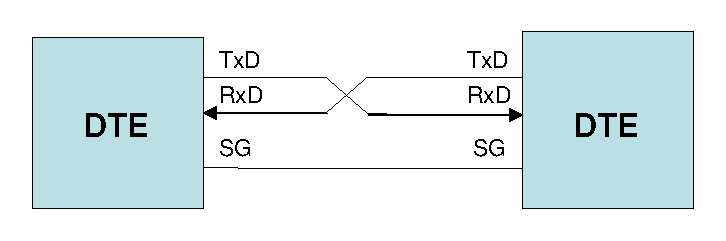
\includegraphics[width=9cm]{./wyklady/RS232_9_2.pdf}\\
		\begin{itemize}
			\item XON – ASCII 19 (CTRL-S)
			\item XOFF – ASCII 17 (CTRL-Q)
		\end{itemize}
	\subsection{Parametry elektryczne}
	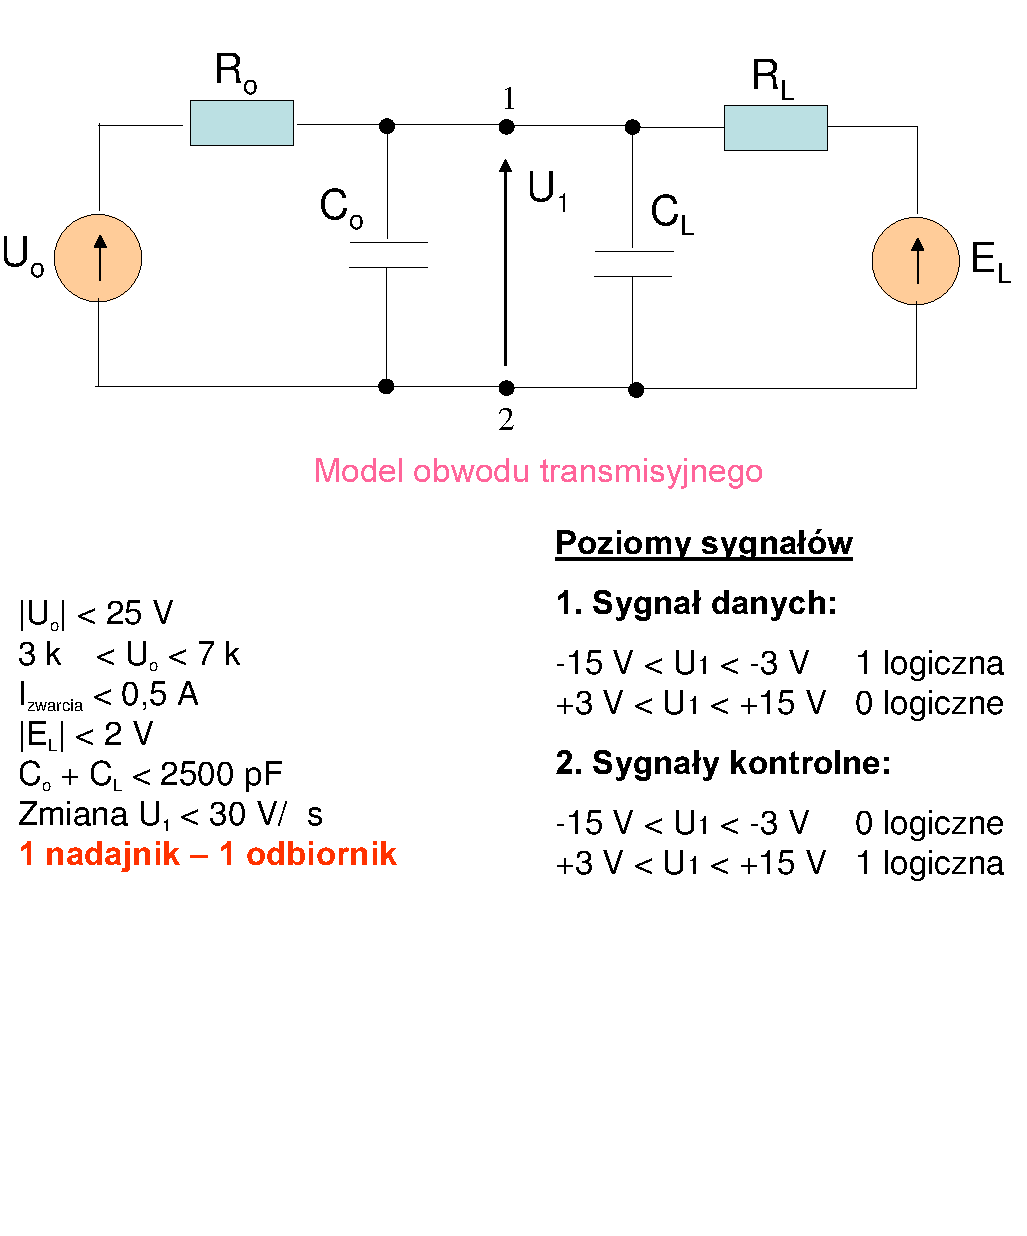
\includegraphics[width=9cm]{./wyklady/RS232_10_1.pdf}
	\subsection{Standardy RS-423, RS-422, RS-485}
		\subsubsection{RS-423A}
		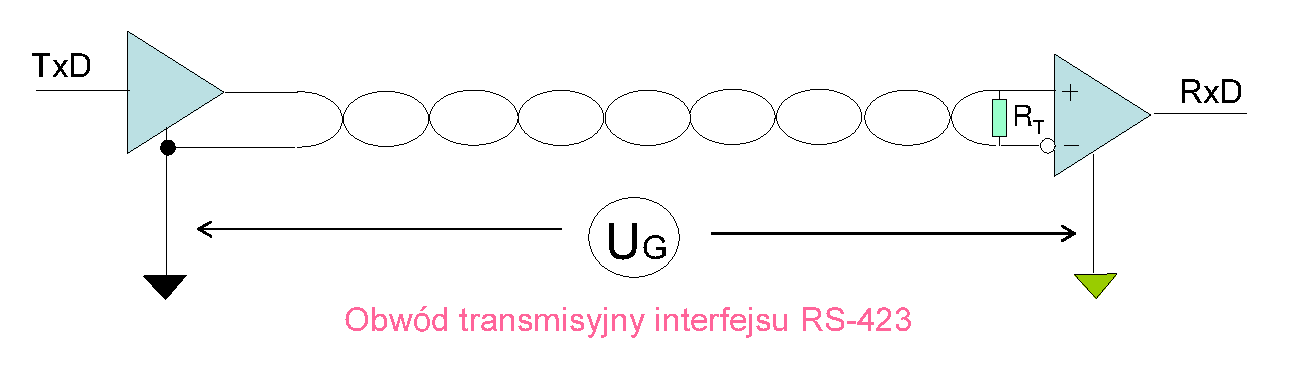
\includegraphics[width=9cm]{./wyklady/RS232_12_1.pdf}
		\begin{itemize}
			\item szybkość do 100 kbd (przy zasięgu do 30 m)
			\item zasięg do 1200 m (przy szybkosci do 3 kbd)
		\end{itemize}
		\subsubsection{RS-422A}
		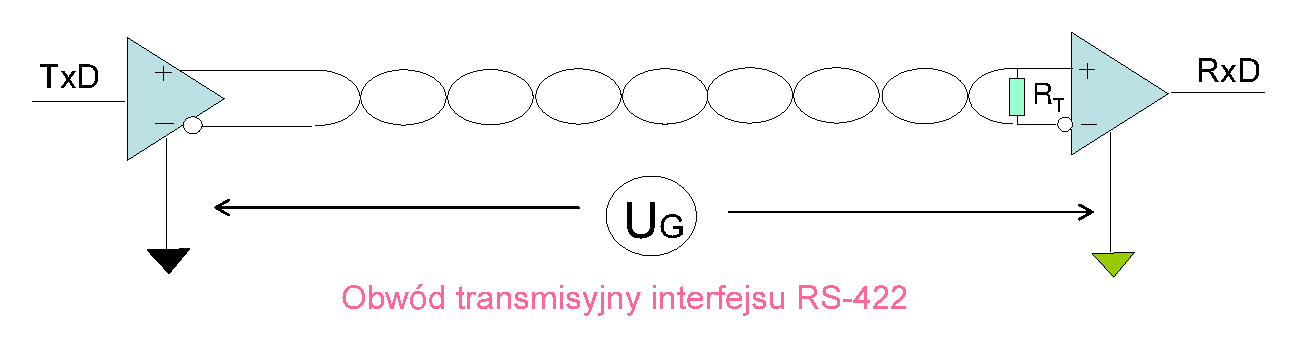
\includegraphics[width=9cm]{./wyklady/RS232_12_2.pdf}
		\begin{itemize}
			\item szybkość do 10 Mbd (przy zasięgu do 100 m)
			\item zasięg do 1200 m (przy szybkości 100 kbd)
		\end{itemize}
		\subsubsection{RS-485A}
		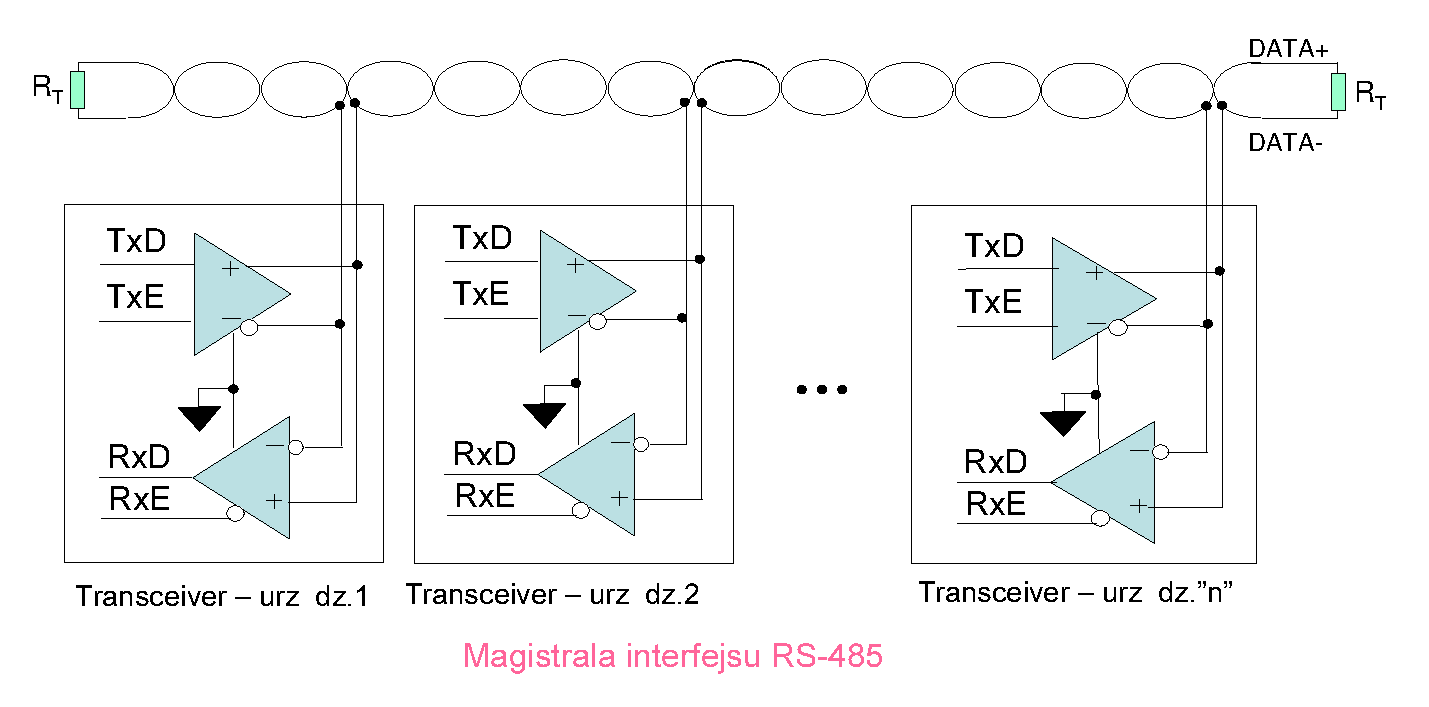
\includegraphics[width=10cm]{./wyklady/RS232_13_1.pdf}
	\subsection{Systemy komunikacyjne oparte na łączu znakowym}
		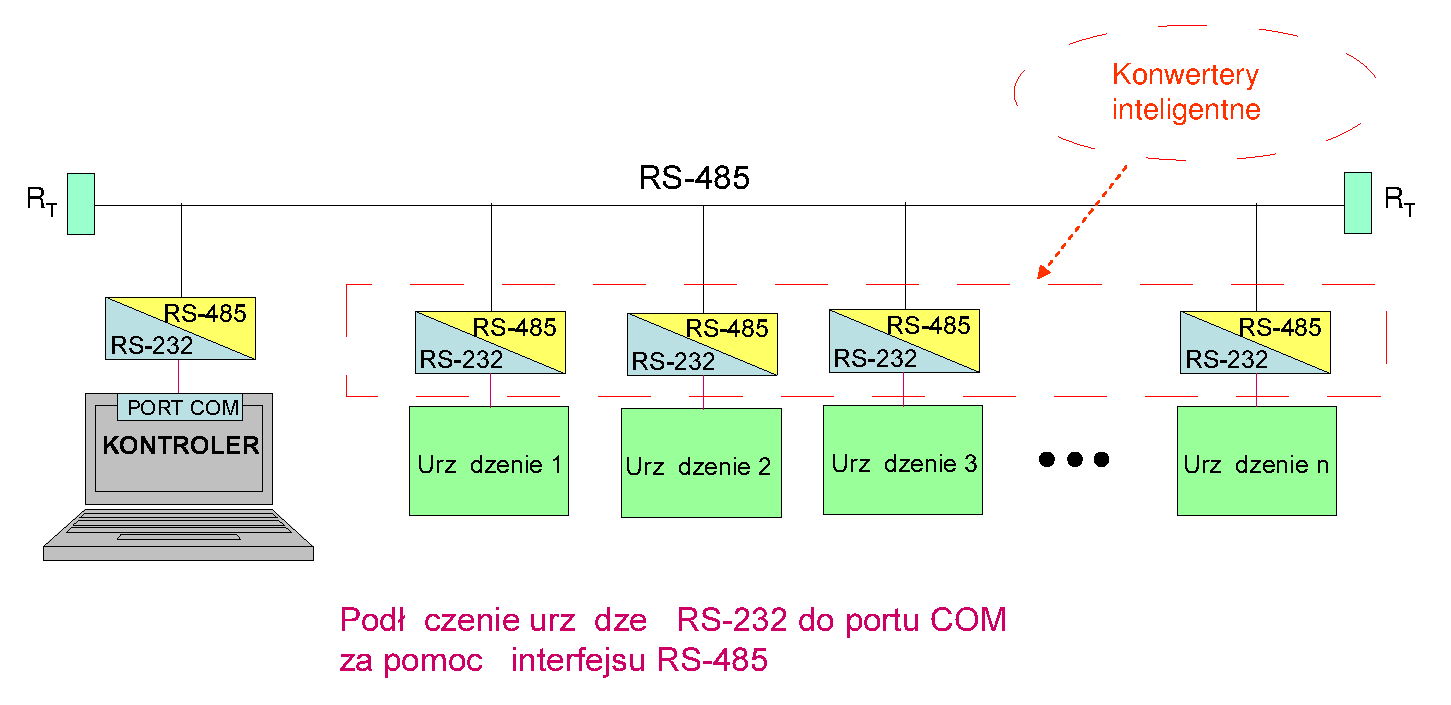
\includegraphics[width=9cm]{./wyklady/RS232_14_1.pdf}\\
		\textbf{Problem}: dostęp do magistrali kontrolera i urządzeń systemu\\
		\textbf{Rozwiązanie}: Implementacja protokołu komunikacyjnego (warstwa łącza danych)\\
		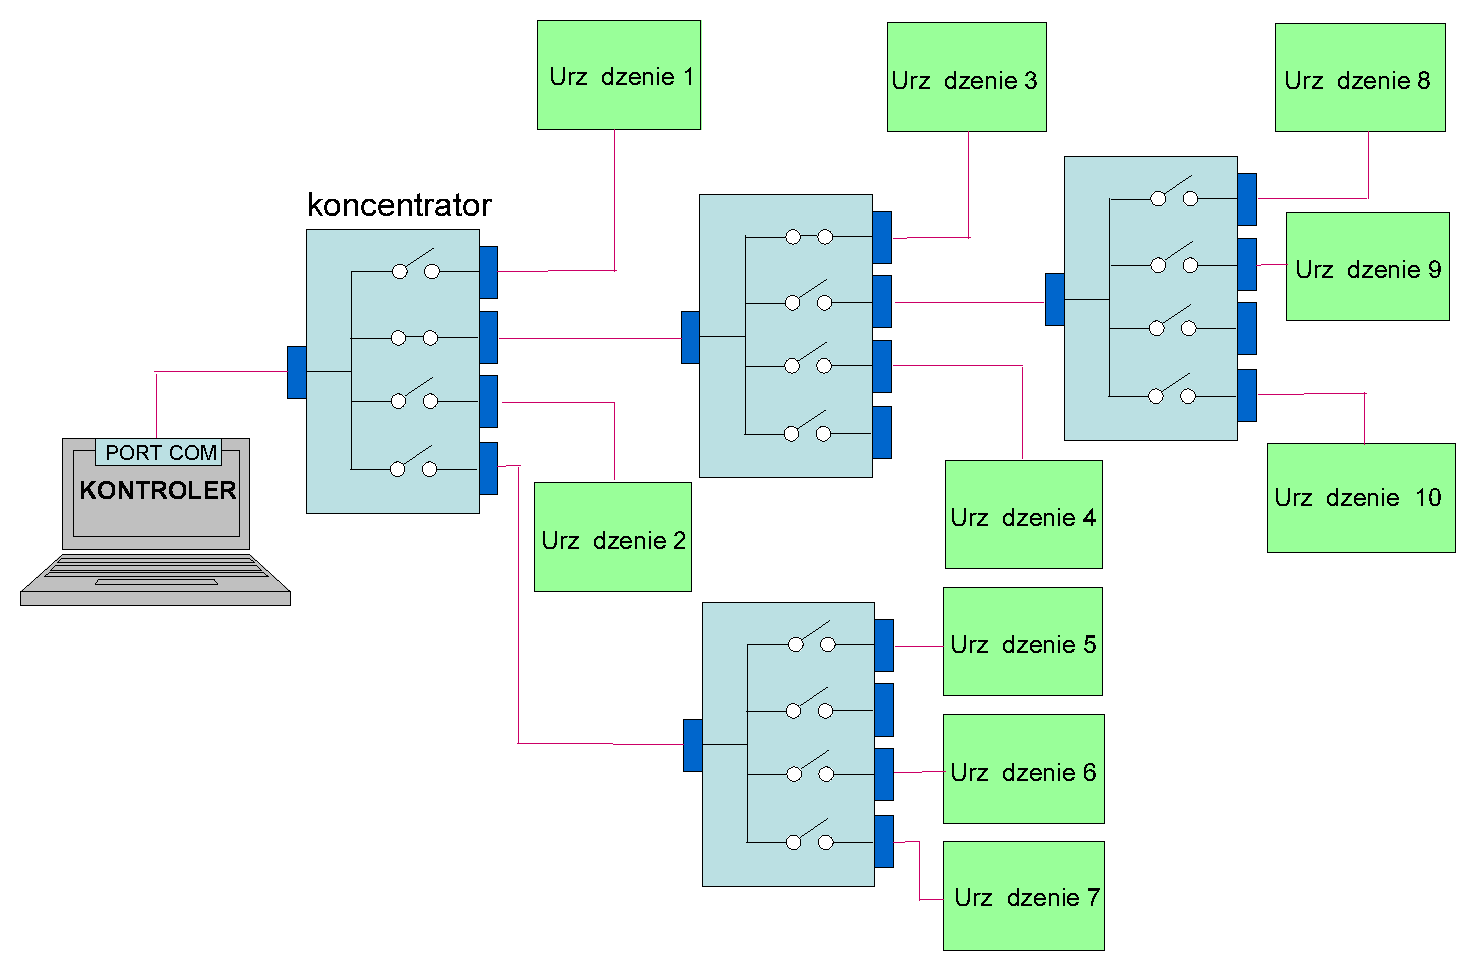
\includegraphics[width=10cm]{./wyklady/RS232_15_1.pdf}\\
	\subsection{System MODBUS}
		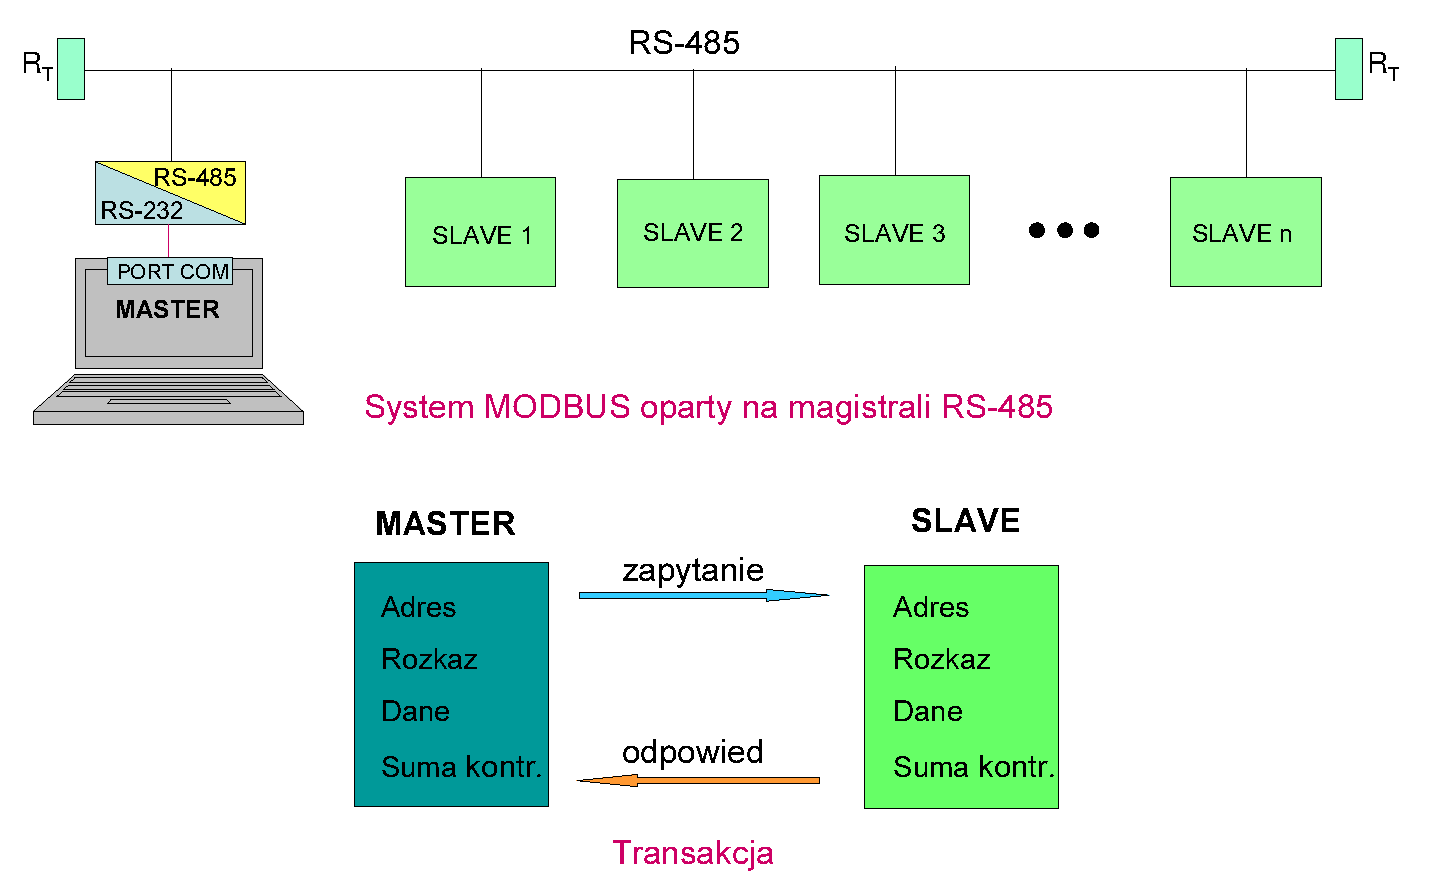
\includegraphics[width=9cm]{./wyklady/RS232_16_1.pdf}\\
		\subsubsection{Rodzaje transakcji}
			\begin{itemize}
				\item adresowana
				\item rozgłoszeniowa
			\end{itemize}
		\subsubsection{Rodzaje odpowiedzi}
			\begin{itemize}
				\item normalna
				\item szczególna
			\end{itemize}
		\subsubsection{Parametry protokołu}
			\begin{itemize}
				\item reguła dostępu do łącza: Master-Slave
				\item zakres adresów: 1 - 247
				\item adres rozgłoszeniowy: 0
				\item kontrola błędów: LRC/CRC, ograniczenie czasowe odpowiedzi
				\item wymagana ciągłość przesyłania znaków w ramce
			\end{itemize}
		\subsubsection{Rodzaje transmisji ramek}
			\begin{itemize}
				\item ASCII
				\item RTU
			\end{itemize}
			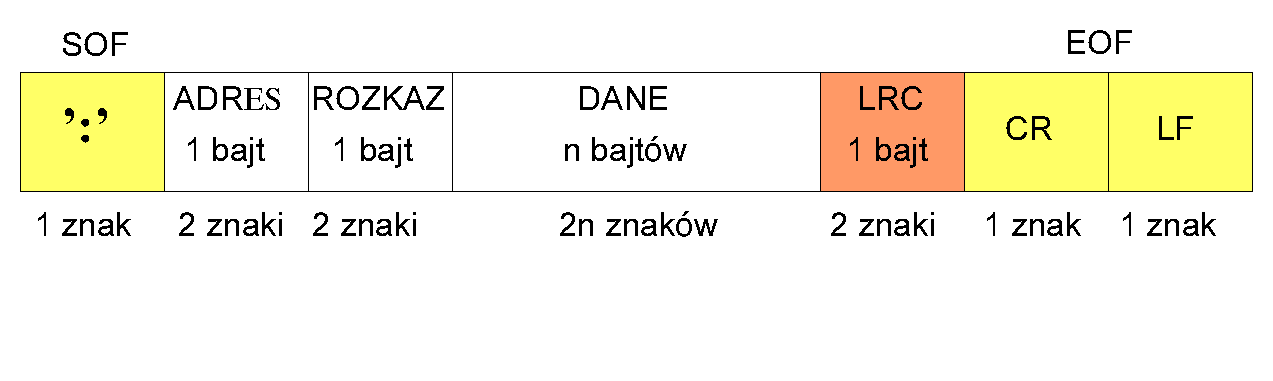
\includegraphics[width=10cm]{./wyklady/RS232_18_1.pdf}
		\subsubsection{Warstwa fizyczna}
		\begin{itemize}
			\item asynchroniczna transmisja znakowa
			\item Formaty znaków
			\begin{itemize}
				\item Tryb ASCII: 7E1, 7O1, 7N2
				\item Tryb RTU: 8E1, 8O1, 8N2
			\end{itemize}
			\item Szybkość: od 1200 bd do 19200 bd
			\item Rodzaj łącza:
			\begin{itemize}
				\item Magistrala RS-485
				\item Multipleksowany RS-232
			\end{itemize}
			\item Rodzaj transmisji (zależny od łącza):
			\begin{itemize}
				\item różnicowa dla RS-485
				\item odniesiona do masy dla RS-232
			\end{itemize}
		\end{itemize}
			
		
	\subsection{Kontroler RS-232 w komputerze PC}
	
	


\section{USB – Uniwersalny interfejs szeregowy}


\section{IEEE-488 and SCPI standards}


\section{IEEE-1394 (FireWire)}


\section{Tłumienie zakłóceń w rozproszonych systemach komputerowych}

\end{document}